Now having two models for the predictions of two organelles: nuclei and ER, it is interesting to visualize the predictions together (see Figure \ref{fig:er-combined}). It is clear from the image that ER indeed is located around the nucleus. As one can see, there is a great advantage in the used of \textit{in silico} fluroescence labeling especially for the cases where several cell targets have to be ananlysed. Instead of a expesive and time-consuming procedure for staining several targets at the same time they can be predicted based on one DIC image only.
\begin{figure}[htb]
    \centering
    \setkeys{Gin}{width=\linewidth}
    \centering
        \begin{tabularx}{\textwidth}{YYYY}
            (a)  \textbf{Ground truth} &
            (b)  \textbf{Prediction} &
            (c)  \textbf{Prediction + nuclei} \\
            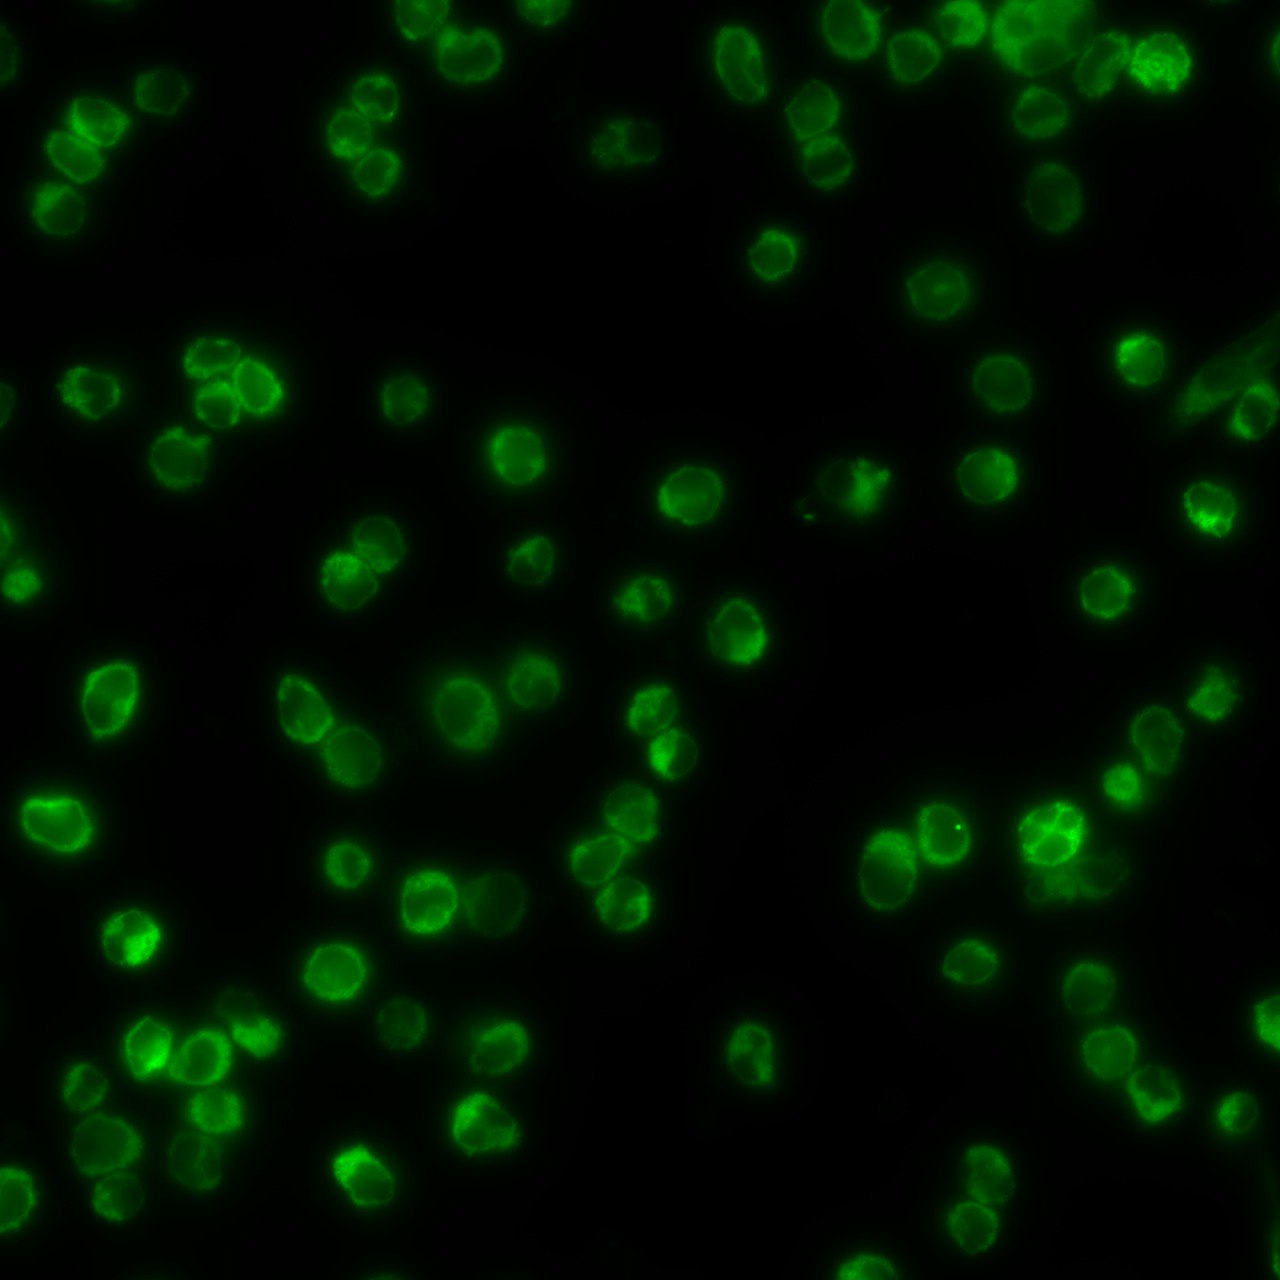
\includegraphics{bilder/ER/gt.jpg} & 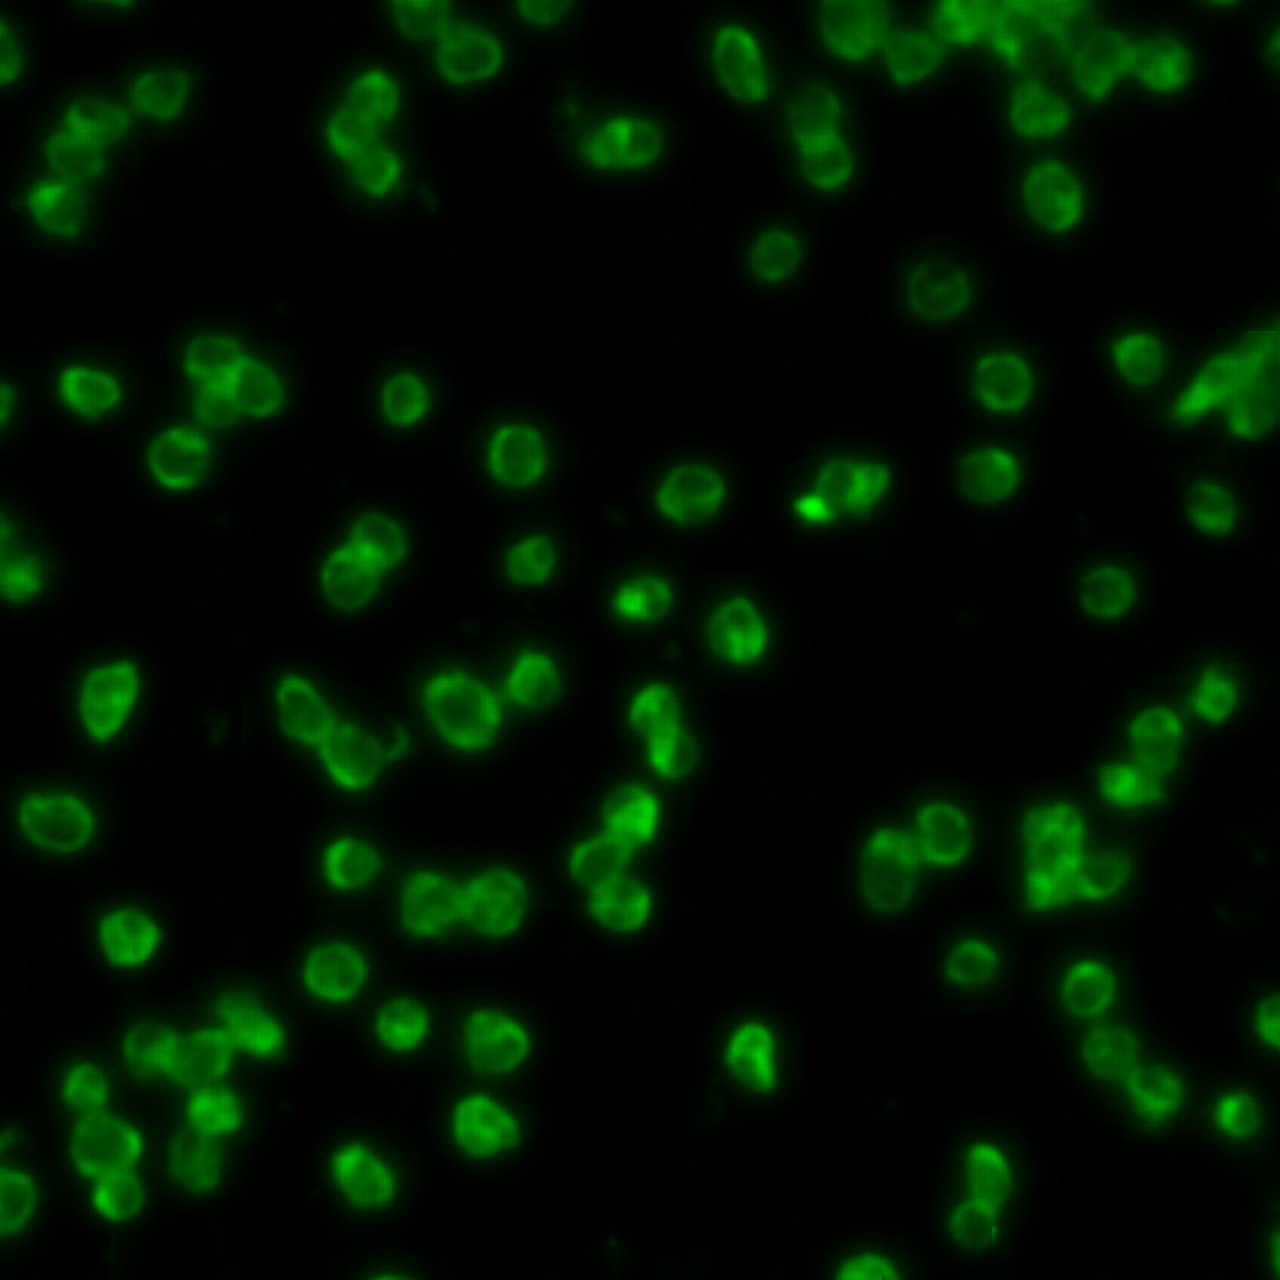
\includegraphics{bilder/ER/er.jpg} &
            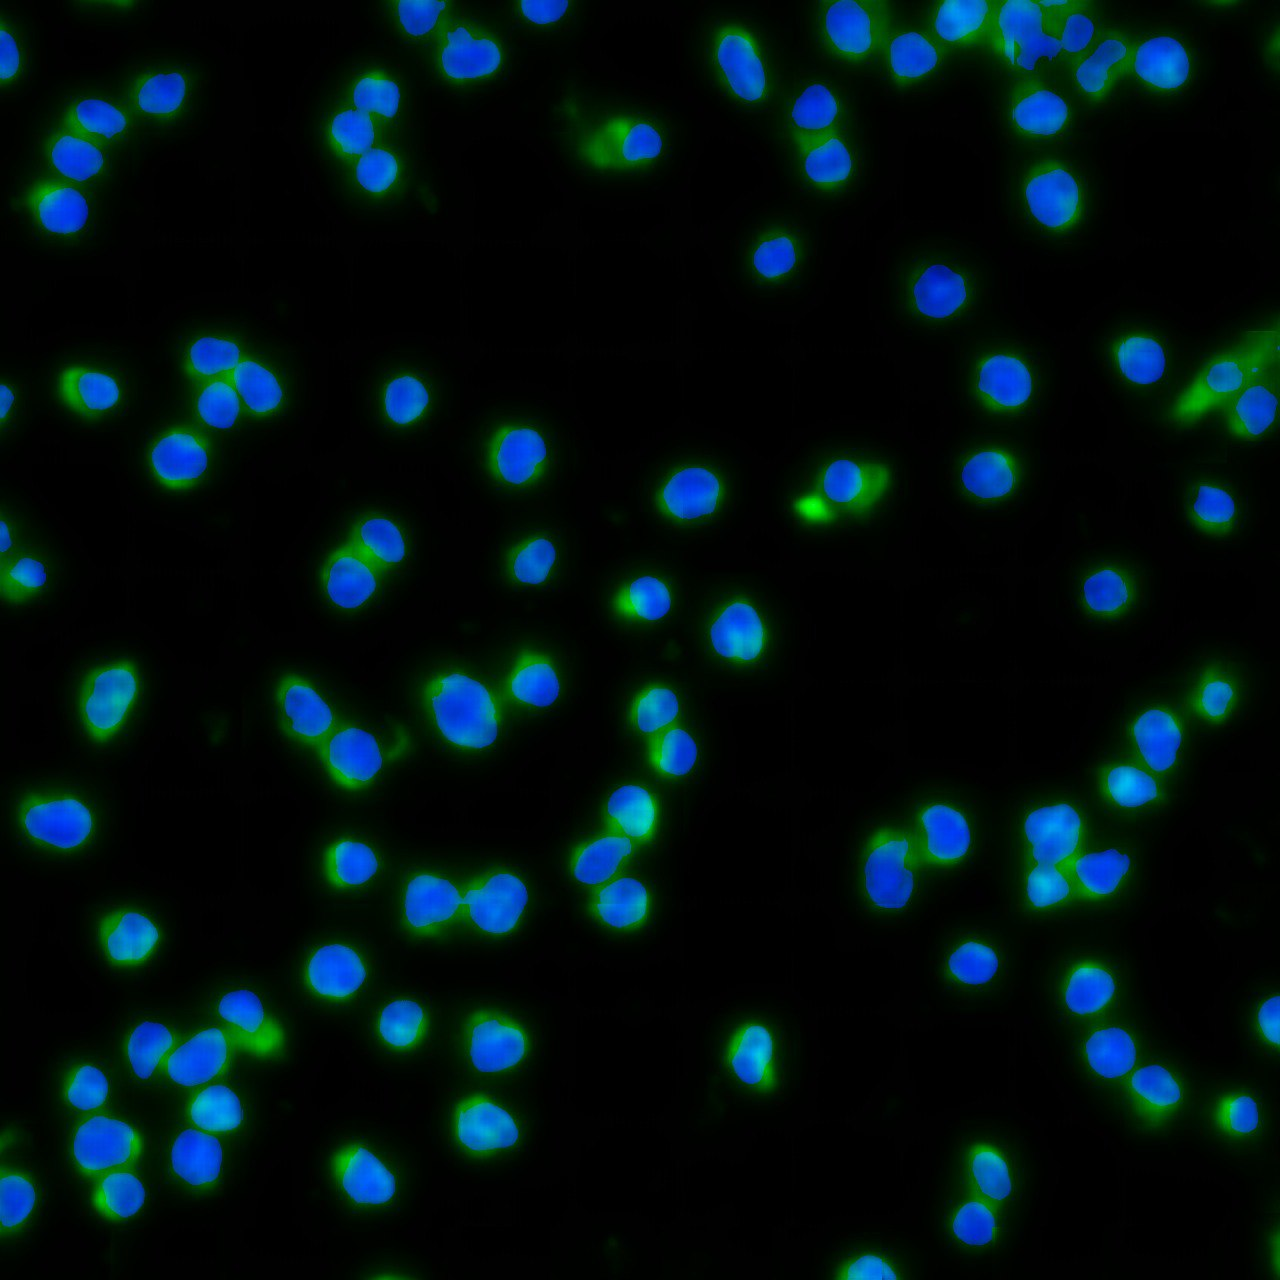
\includegraphics{bilder/ER/gt_nuclei.jpg}
        \end{tabularx}
    \caption{Combination of ER with nuclei prediction. Image (a) here is the original fluorescence image of ER, image (b) is the UNet prediction of ER and image (c) is the combination of predicted ER (green) with predicted nuclei (blue).}
    \label{fig:er-combined}
\end{figure}